\documentclass[tikz,convert=pdf2svg]{standalone}
\usepackage{tikz}
\usetikzlibrary{shapes,positioning,calc}
\begin{document}
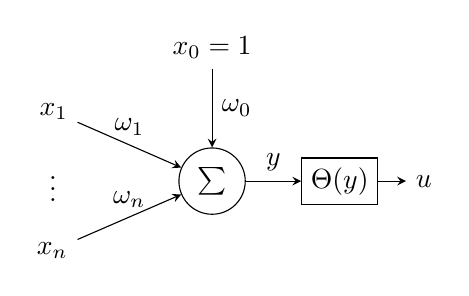
\begin{tikzpicture}[]
    % \node[draw, circle] (neuron) {$\Theta\Big(\sum_{i=0}^n \omega_i  x_i\Big)$};
    \node[draw, circle] (neuron) {$\sum$};
    \node[draw, rectangle,right=2em of neuron] (act)   {$\Theta(y)$};

    \node[above left=1em and 4em of neuron] (x1) {$x_1$};
    \node[below left=1em and 4em of neuron] (xn) {$x_n$};
    \node[above=of neuron] (bias) {$x_0=1$};

    \node at ($(x1)!0.5!(xn)$) {$\vdots$};

    \draw[-stealth] (x1) -- node[above,midway] {$\omega_1$} (neuron);
    \draw[-stealth] (xn) -- node[above,midway] {$\omega_n$} (neuron);
    \draw[-stealth] (bias) -- node[right,midway] {$\omega_0$} (neuron);

    % \node[draw, right=2em of neuron] (act_func) {$\Theta(u)$};
    \node[right=1em of act] (out) {$u$};

    % \draw[-stealth] (neuron) -- node[above,midway] {$u$} (act_func);
    % \draw[-stealth] (act_func) -- (out);
    \draw[-stealth] (neuron) -- node[above,midway]{$y$} (act);
    \draw[-stealth] (act) -- (out);
\end{tikzpicture}
\end{document}
